\documentclass[9pt]{beamer}
\mode<presentation>
{
  \usetheme{Madrid}       % or try default, Darmstadt, Warsaw, ...
  \usecolortheme{default} % or try albatross, beaver, crane, ...
  \usefonttheme{serif}    % or try default, structurebold, ...
  \setbeamertemplate{navigation symbols}{}
  \setbeamertemplate{caption}[numbered]
} 
% Ba Hong adds
\usepackage[symbol*]{footmisc}
\DefineFNsymbolsTM{myfnsymbols}{% def. from footmisc.sty "bringhurst" symbols
  \textasteriskcentered *
  \textdagger    \dagger
  \textdaggerdbl \ddagger
  \textsection   \mathsection
  \textbardbl    \|%
  \textparagraph \mathparagraph
}%
\AtBeginSection[]
{
  \begin{frame}
    \frametitle{Table of Contents}
    \tableofcontents[currentsection]
  \end{frame}
}
\usepackage{subfig,booktabs,hyperref,amsmath,amsxtra,amssymb,latexsym,amscd,amsthm,amsfonts,graphicx}
\usepackage[english]{babel}
\numberwithin{equation}{section}
\renewcommand\thempfootnote{\arabic{mpfootnote}}
\usepackage[utf8x]{inputenc}
\usepackage{pgfpages}
\pgfpagesuselayout{resize to}[%
  physical paper width=8in, physical paper height=6in]

\title[Seminar Math Modelling]{\Huge Explicit Runge Kutta Methods}
\author{\textsc{Hong N. Q. B.},  \textsc{Tung D. T. N.}, \textsc{Thinh N. A.} }
\date{\today}
\newcommand{\mytab}{
  \begin{tabular}{}
    \toprule
    One & Two & Three \\
    \midrule
    $x$ & $y$ & $z$ \\
    1 & 2 & 3 \\
    \bottomrule
  \end{tabular}
}
\begin{document}

\begin{frame}
  \titlepage
\end{frame}
\begin{frame}{Outline}
  \tableofcontents
\end{frame}
\section{Obstables}
\subsection{How to Solve ODEs, PDEs Practically/Generally}
\begin{frame}{Solve ODEs and PDEs analytically vs. numerically.}
\begin{itemize}
\item ``There is \textbf{no general theory known} concerning the \textbf{solvability of all partial differential equations}. Such a theory is \textbf{extremely unlikely to exist}, given the rich variety of physical, geometric, and probabilistic  phenomena which can be modeled by PDE.'' - L. C. Evans.
\vspace{0.2cm}
\item \textbf{Numerical solutions} are usually assigned to physical situations and as a result \textbf{require a lot of background information} on the type of DEs in order to solve.
\end{itemize}
\end{frame}


\subsection{Accuracy and Efficiency in Numerical Schemes}
\begin{frame}{Accuracy and Efficiency.}
Although we can solve ODEs and PDEs numerically, many practical problems rise then.
\begin{block}{Accuracy and Efficiency Problems}
\textbf{Accuracy} and \textbf{efficiency} in a particular numerical scheme.
\begin{itemize}
\item Partial differentials and systems can be solved with \textbf{FDM, FVM} and \textbf{FEM.}
\vspace{0.2cm}
\item Most equations can be solved some level of accuracy, but are \textbf{computationally expensive} - \textbf{lots of processing time} \textbf{(Efficiency Problems).}
\end{itemize}
\end{block}
and especially \textbf{Stiffness Problems.}

\end{frame}

\begin{frame}{Stiffness Problems.}
\begin{figure}
\centering 
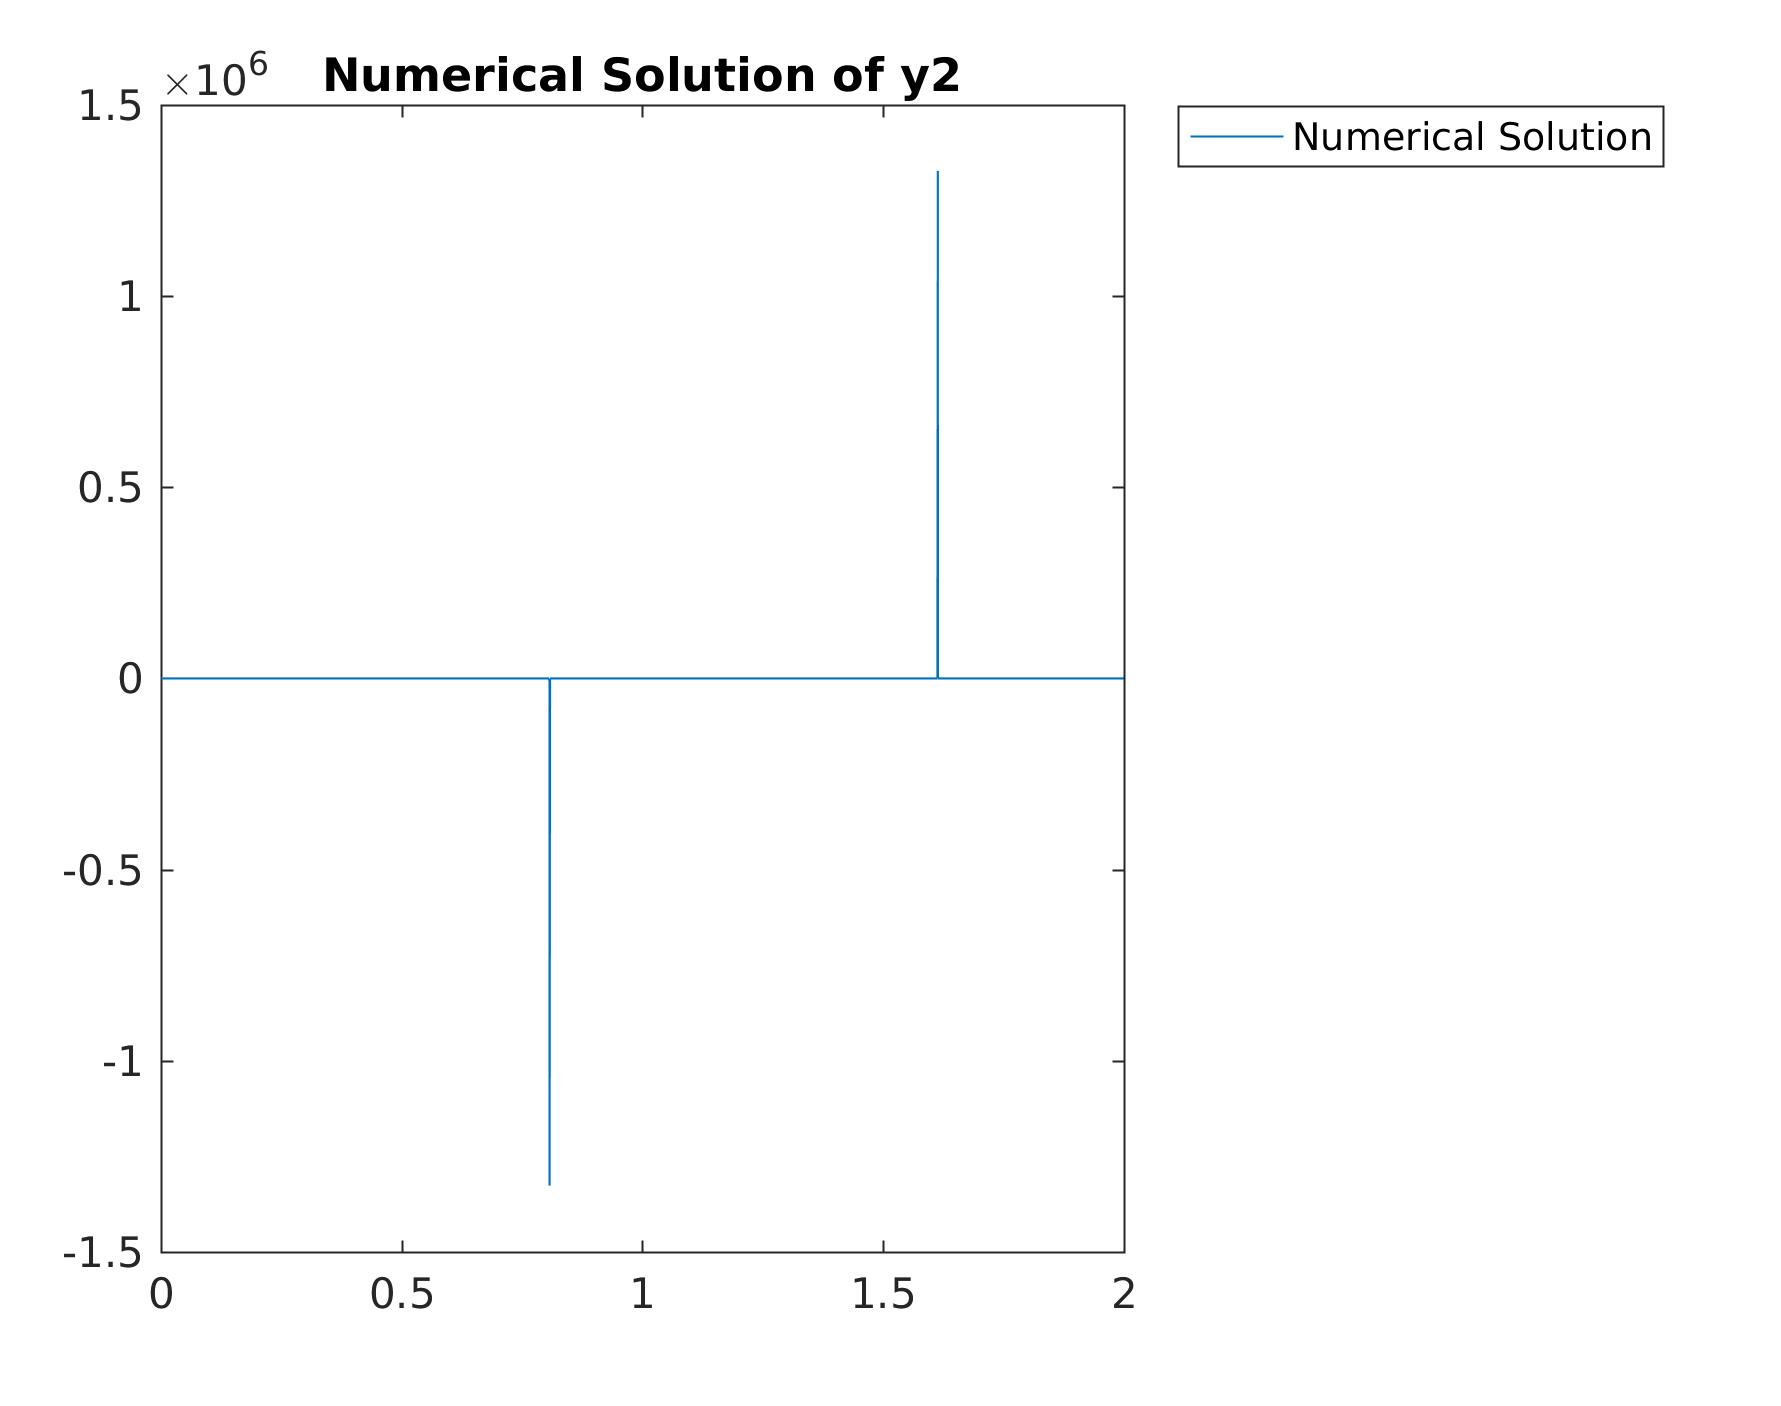
\includegraphics[scale=0.15]{ats_vdp_y2}
\caption{\textbf{\textsf{Stiffness Problems.}}}
\end{figure}
\end{frame}

\section{Explicit Runge Kutta Methods}
\begin{frame}{Introduction to Runge Kutta Methods.}
\begin{itemize}
\item \textbf{Classic, popular, well-known} methods.
\item Are a family of \textbf{explicit and implicit iterative methods} for the approximate solutions of ODEs.
\item \textbf{Extremely powerful tools} for the solution of ODEs.
\item One can solve a \textbf{majority of ODEs} using a Runge-Kutta scheme.
\end{itemize}
\end{frame}

\subsection{General Form of Explicit Runge Kutta Method}
\begin{frame}{General Form of Explicit Runge Kutta Method}
\begin{block}{Definition of explicit Runge Kutta methods.}
The family of explicit Runge Kutta methods is given by
\begin{align}
\label{2.1}
{y^{\left( {n + 1} \right)}} = {y^{\left( n \right)}} + h\sum\limits_{i = 1}^s {{b_i}{k_i}} 
\end{align}
where ${k_i} = f\left( {{\tau _i},{\eta _i}} \right), i = 1,2, \ldots ,s$ with 
\begin{align}
\label{2.2}
{\tau _i} &= {t_n} + {c_i}h\\
{\eta _i} &= {y_n} + \sum\limits_{j = 1}^{i - 1} {{a_{ij}}{k_j}} \label{2.3}
\end{align}
\end{block}
\textbf{\textsf{Notations.}} $s$ (the number of stages), $a_{ij},1\le j<i \le s$, $b_i$, $i=1,2,\ldots,s$ and $c_i,i=2,3,\ldots,s$ (the coefficients), $A=\left[a_{ij}\right]$ (the Runge Kutta matrix) and $b_i$ (weights), $c_i$ (nodes).

\end{frame}

\begin{frame}{Butcher Tableau.}
\begin{block}{Consistent Runge Kutta method}
The Runge Kutta method is \textbf{consistent} if 
\begin{align}
\sum\limits_{j = 1}^{i - 1} {{a_{ij}}}  = {c_i},i = 2, \ldots ,s
\end{align}
\end{block}
\begin{block}{Butcher tableau.}
These data are usually arranged in a \textbf{Butcher tableau.}
\begin{align}
\begin{array}{*{20}{c}}
0&\vline& {}&{}&{}&{}&{}\\
{{c_2}}&\vline& {{a_{21}}}&{}&{}&{}&{}\\
{{c_3}}&\vline& {{a_{31}}}&{{a_{32}}}&{}&{}&{}\\
 \vdots &\vline&  \vdots & \vdots & \ddots &{}&{}\\
{{c_s}}&\vline& {{a_{s1}}}&{{a_{s2}}}& \cdots &{{a_{s,s - 1}}}&{}\\
\hline
{}&\vline& {{b_1}}&{{b_2}}& \cdots &{{b_{s - 1}}}&{{b_s}}
\end{array}
\end{align}
\end{block}
\end{frame}

\subsection{Practical Problems (Stiffness)}
\begin{frame}{van der Pol Stiffness Problem.}
\begin{columns}[t]
\column{.5\textwidth}
\centering
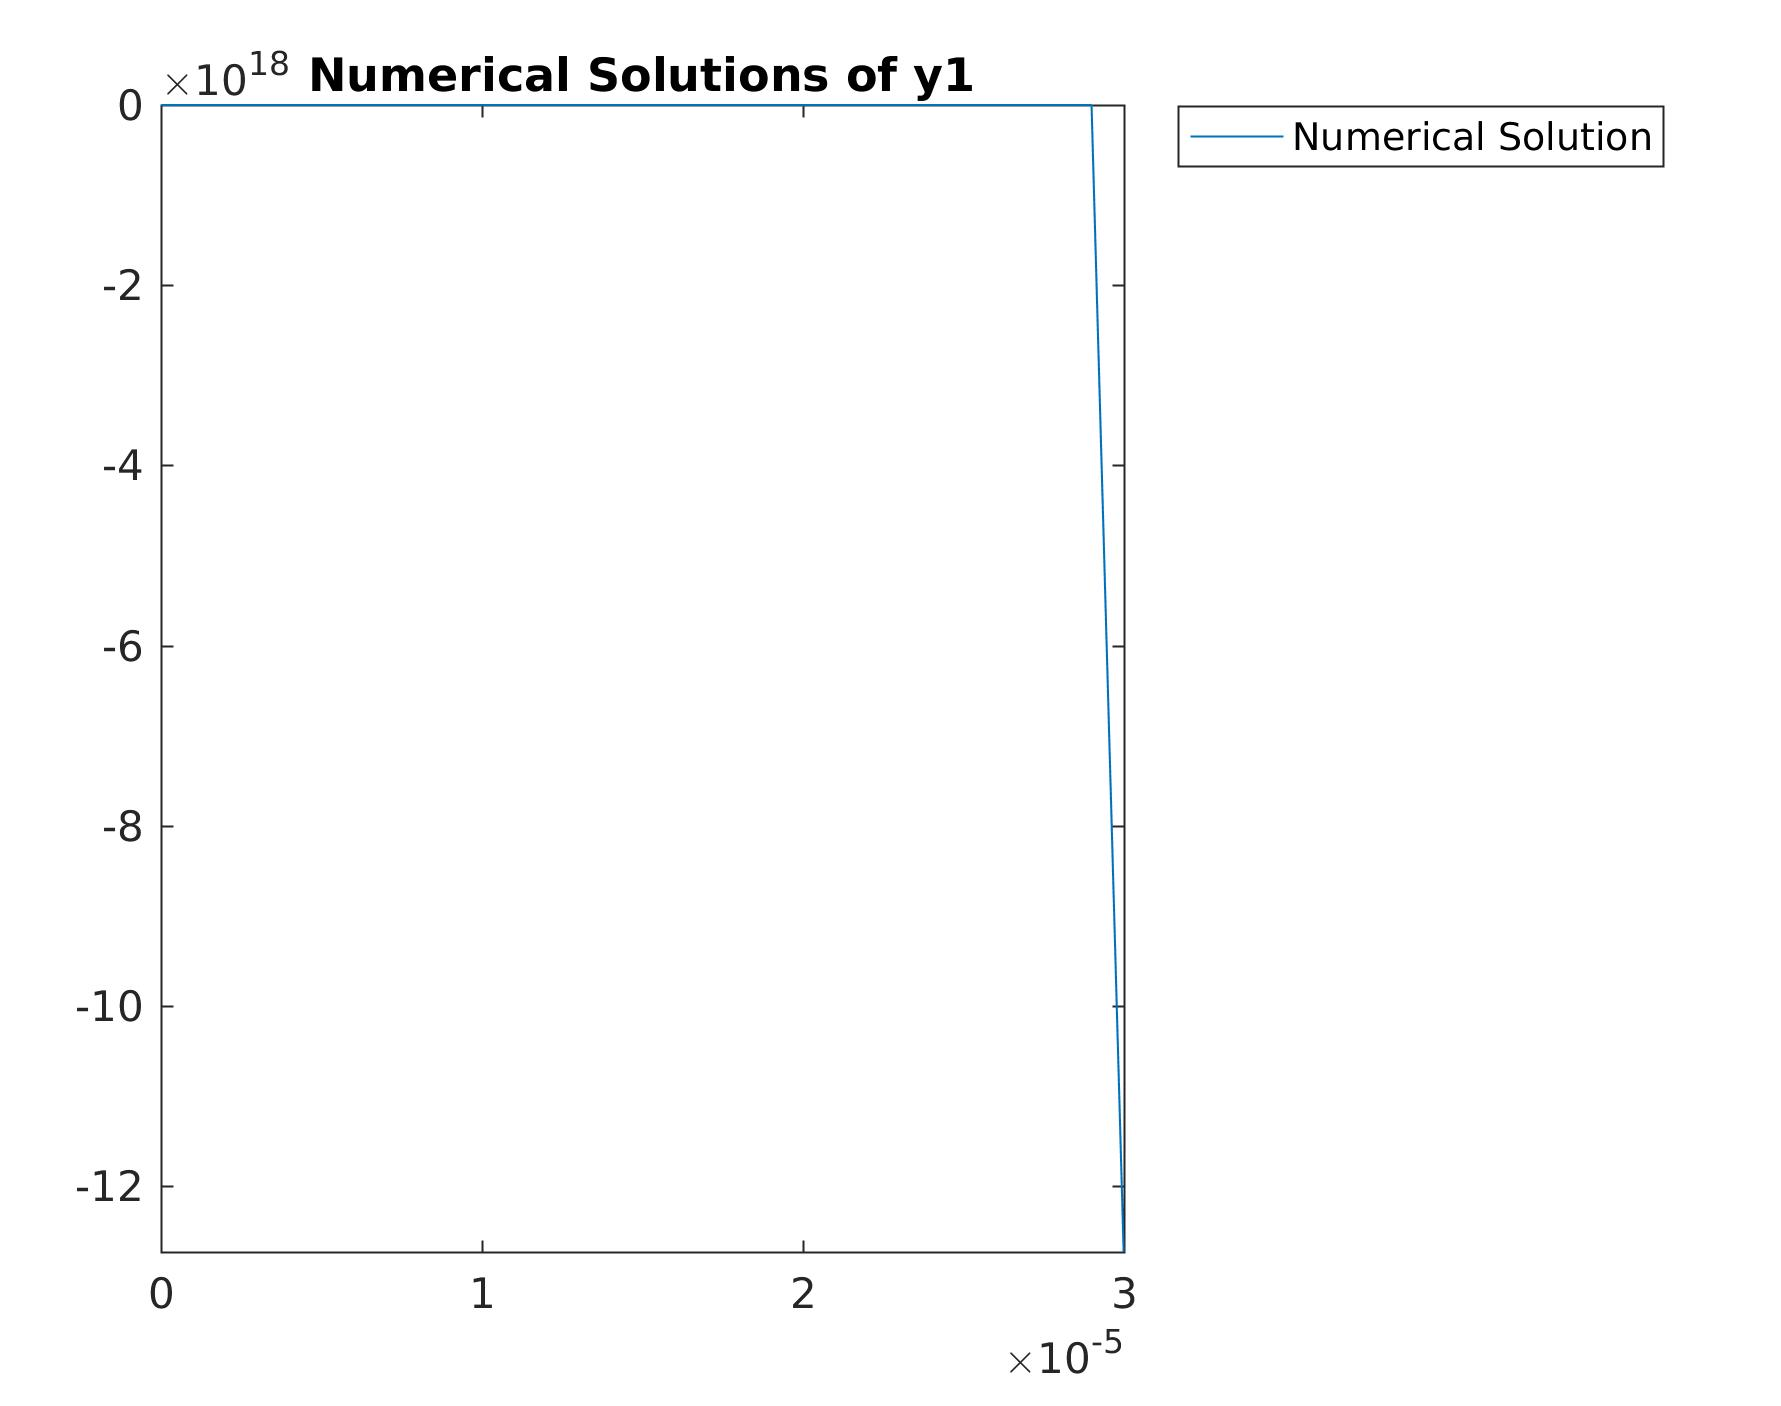
\includegraphics[scale=0.151]{fts_vdp_y1_1e-6}
\column{.5\textwidth}
\centering
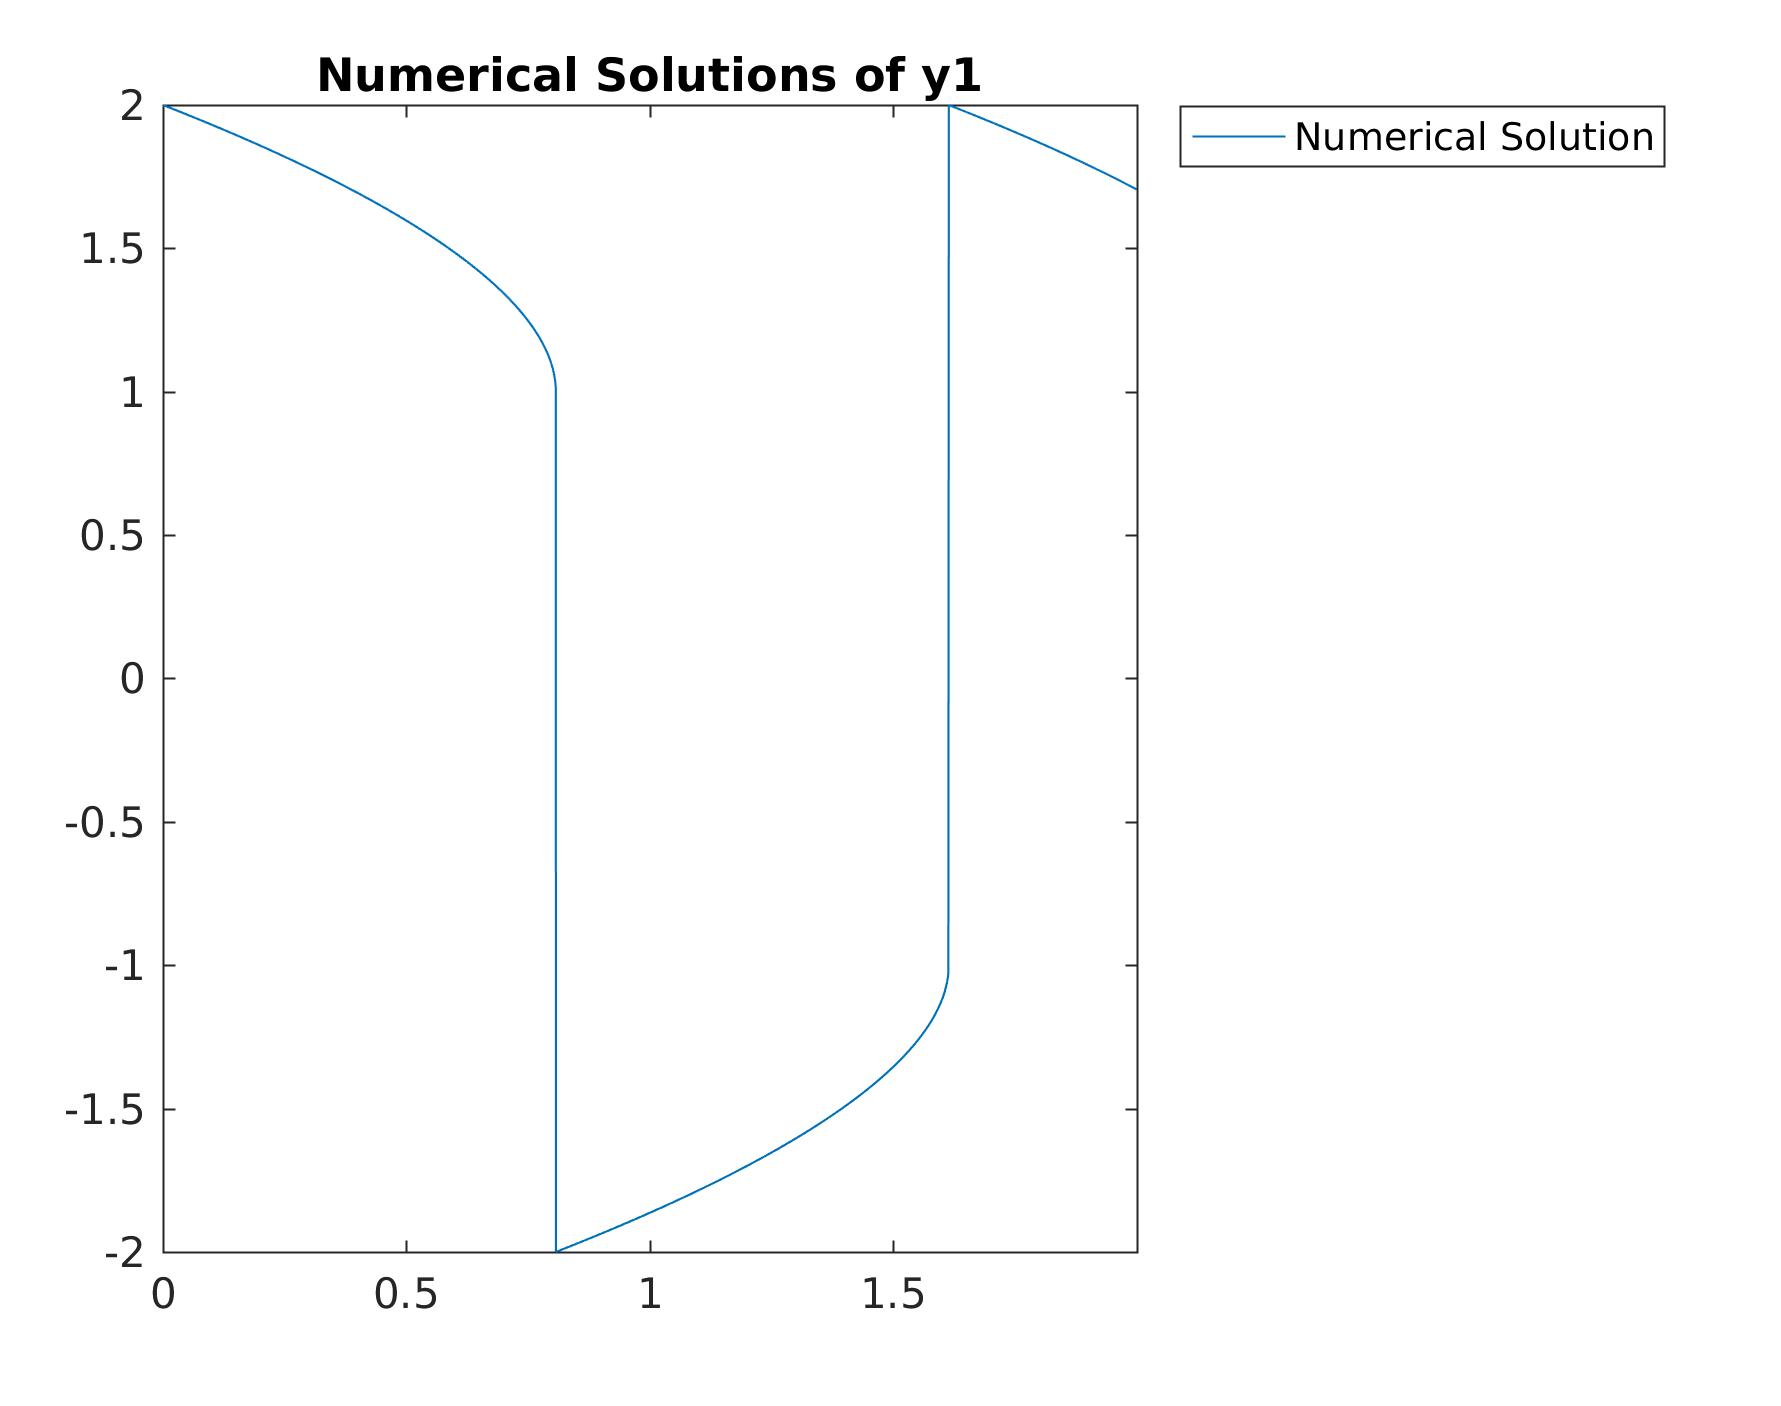
\includegraphics[scale=0.151]{fts_vdp_y1_1e-7}
\end{columns}

\end{frame}

\section{Adaptive Time Steps Algorithm (explicit RK)}
\begin{frame}{An Adaptive Time Step Algorithm.}
\begin{itemize}
\item Adaptive Time Steps Scheme is \textbf{not well-known.}
\item There are \textbf{lots of Adaptive Time Step Schemes.}
\item An adaptive time steps algorithm for explicit Runge Kutta method can be found in the following article.
\end{itemize}
\begin{alertblock}{Article.}
Tan Trung Nguyen, Frédérique Laurent, Rodney Fox, Marc Massot. \textit{Solution of population balance equations in applications with fine particles: mathematical modeling and numerical schemes}. 2016. $<$hal-01247390v2$>$
\end{alertblock}


\end{frame}



\section{Applications}
\begin{frame}{Curtiss-Hirchfelder Equation.}
\textbf{\textsf{Applications.}} Used to test numerical methods for the solution of ODEs.
\begin{block}{Curtiss-Hirchfelder equation.}
\begin{align}
\frac{{dy}}{{dt}} &=  - 50\left( {y - \cos \left( t \right)} \right)\\
y\left( 0 \right) &= 1
\end{align}
\end{block}
\end{frame}

\begin{frame}
\begin{figure}
\centering
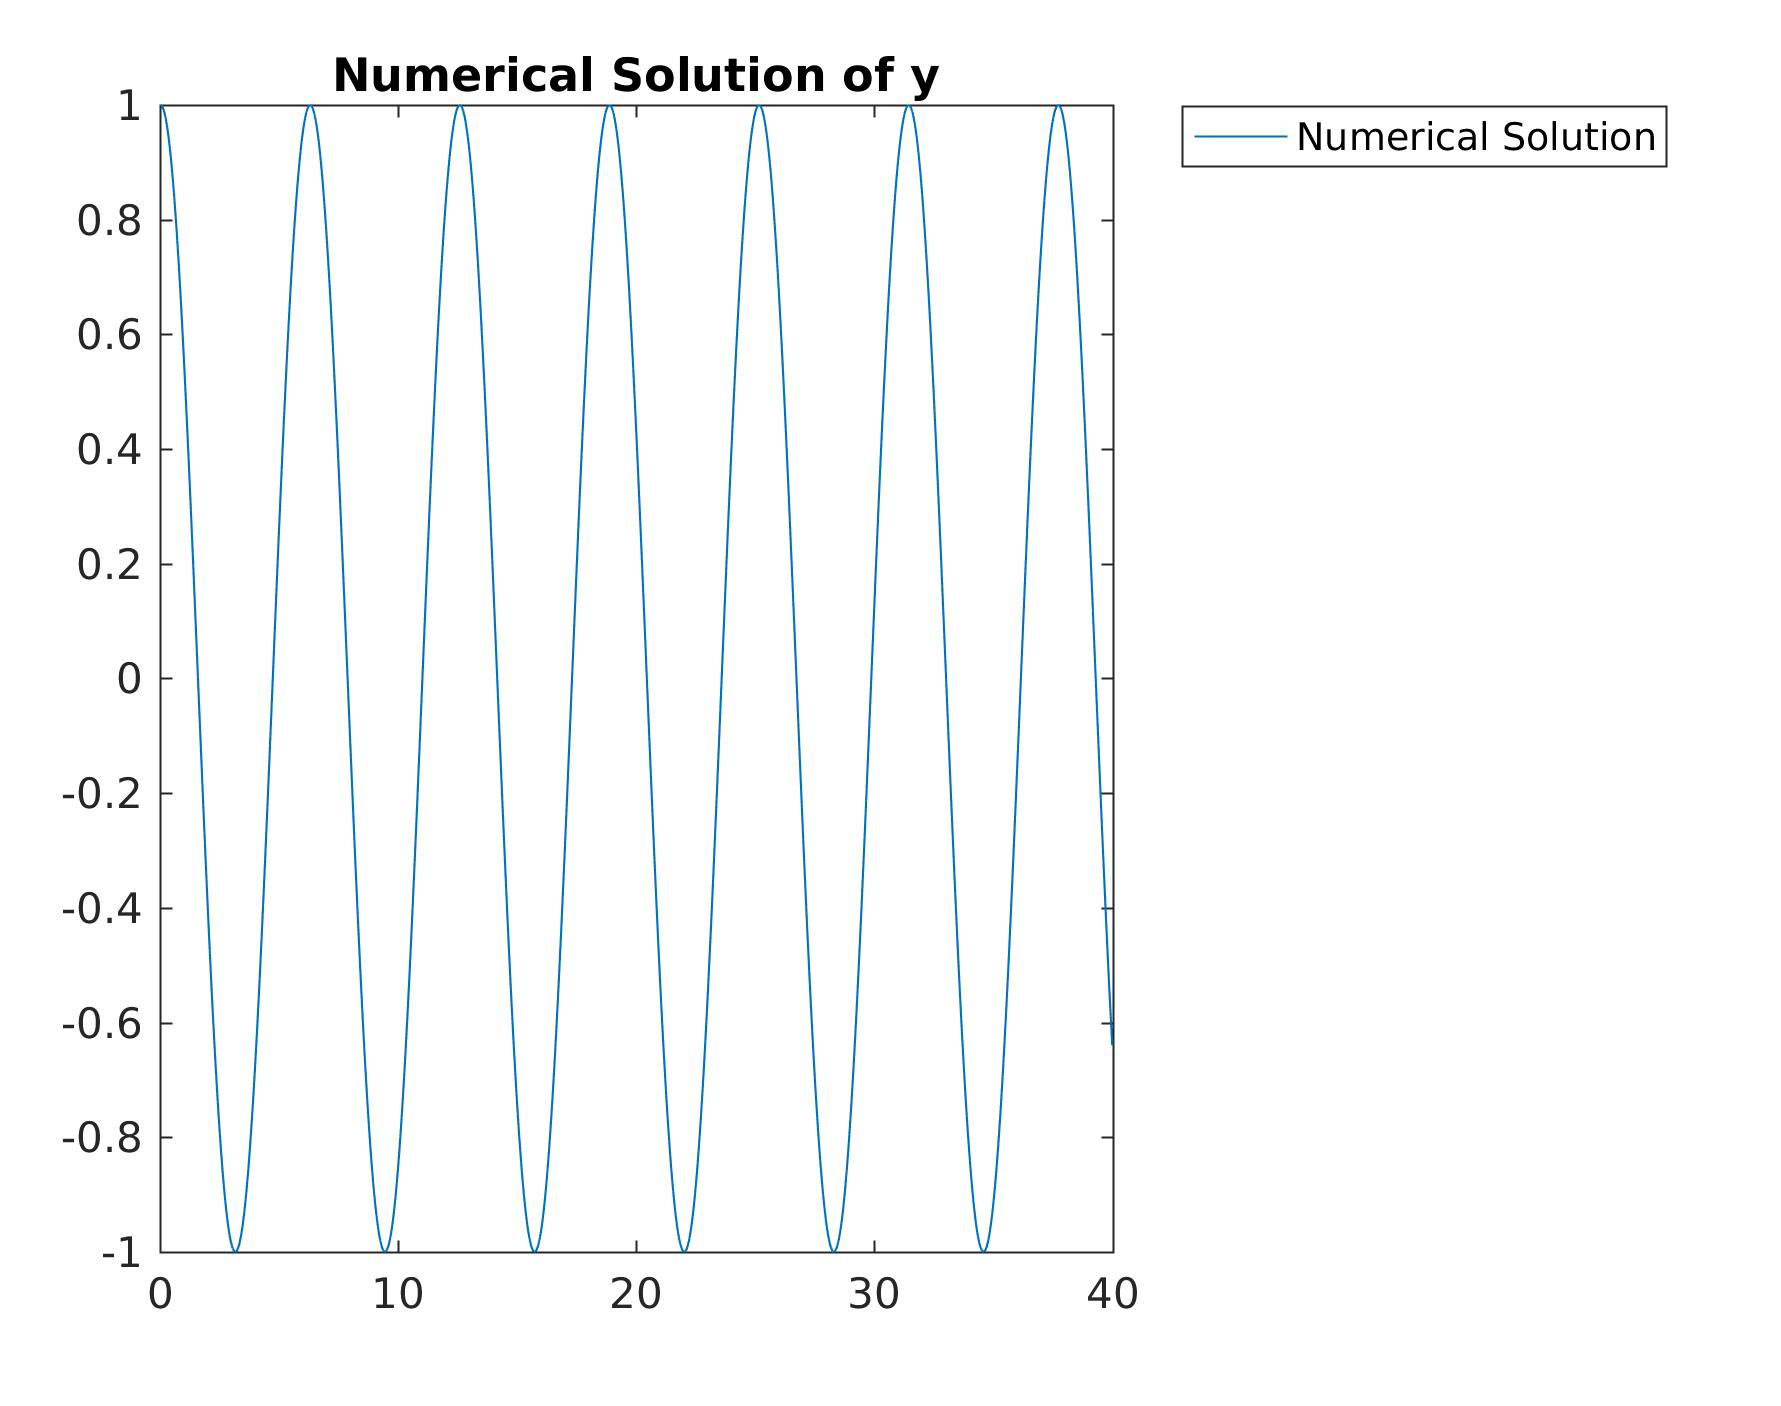
\includegraphics[scale=0.15]{ats_ch_y_1}
\caption{Using Adaptive Time Steps for Curtiss-Hirschfelder equation.}
\end{figure}
\end{frame}


\begin{frame}{Brusselator.}
\textbf{\textsf{Applications.}}
\begin{itemize}
\item A theoretical model for a type of \textbf{autocatalytic reaction.}
\end{itemize}
\begin{block}{Brusselator.}
\begin{subequations}
\begin{align}
    \frac{dy_1}{dt}  &=  1 - 4y_1 + y_1^2 y_2
    \\
    \frac{dy_2}{dt}  &=  3y_1 - y_1^2 y_2
\end{align}
\end{subequations}
where $y_1(0) = 1$ and $y_2(0) = 1$.
\end{block}
\end{frame}

\begin{frame}
\begin{figure}
\centering
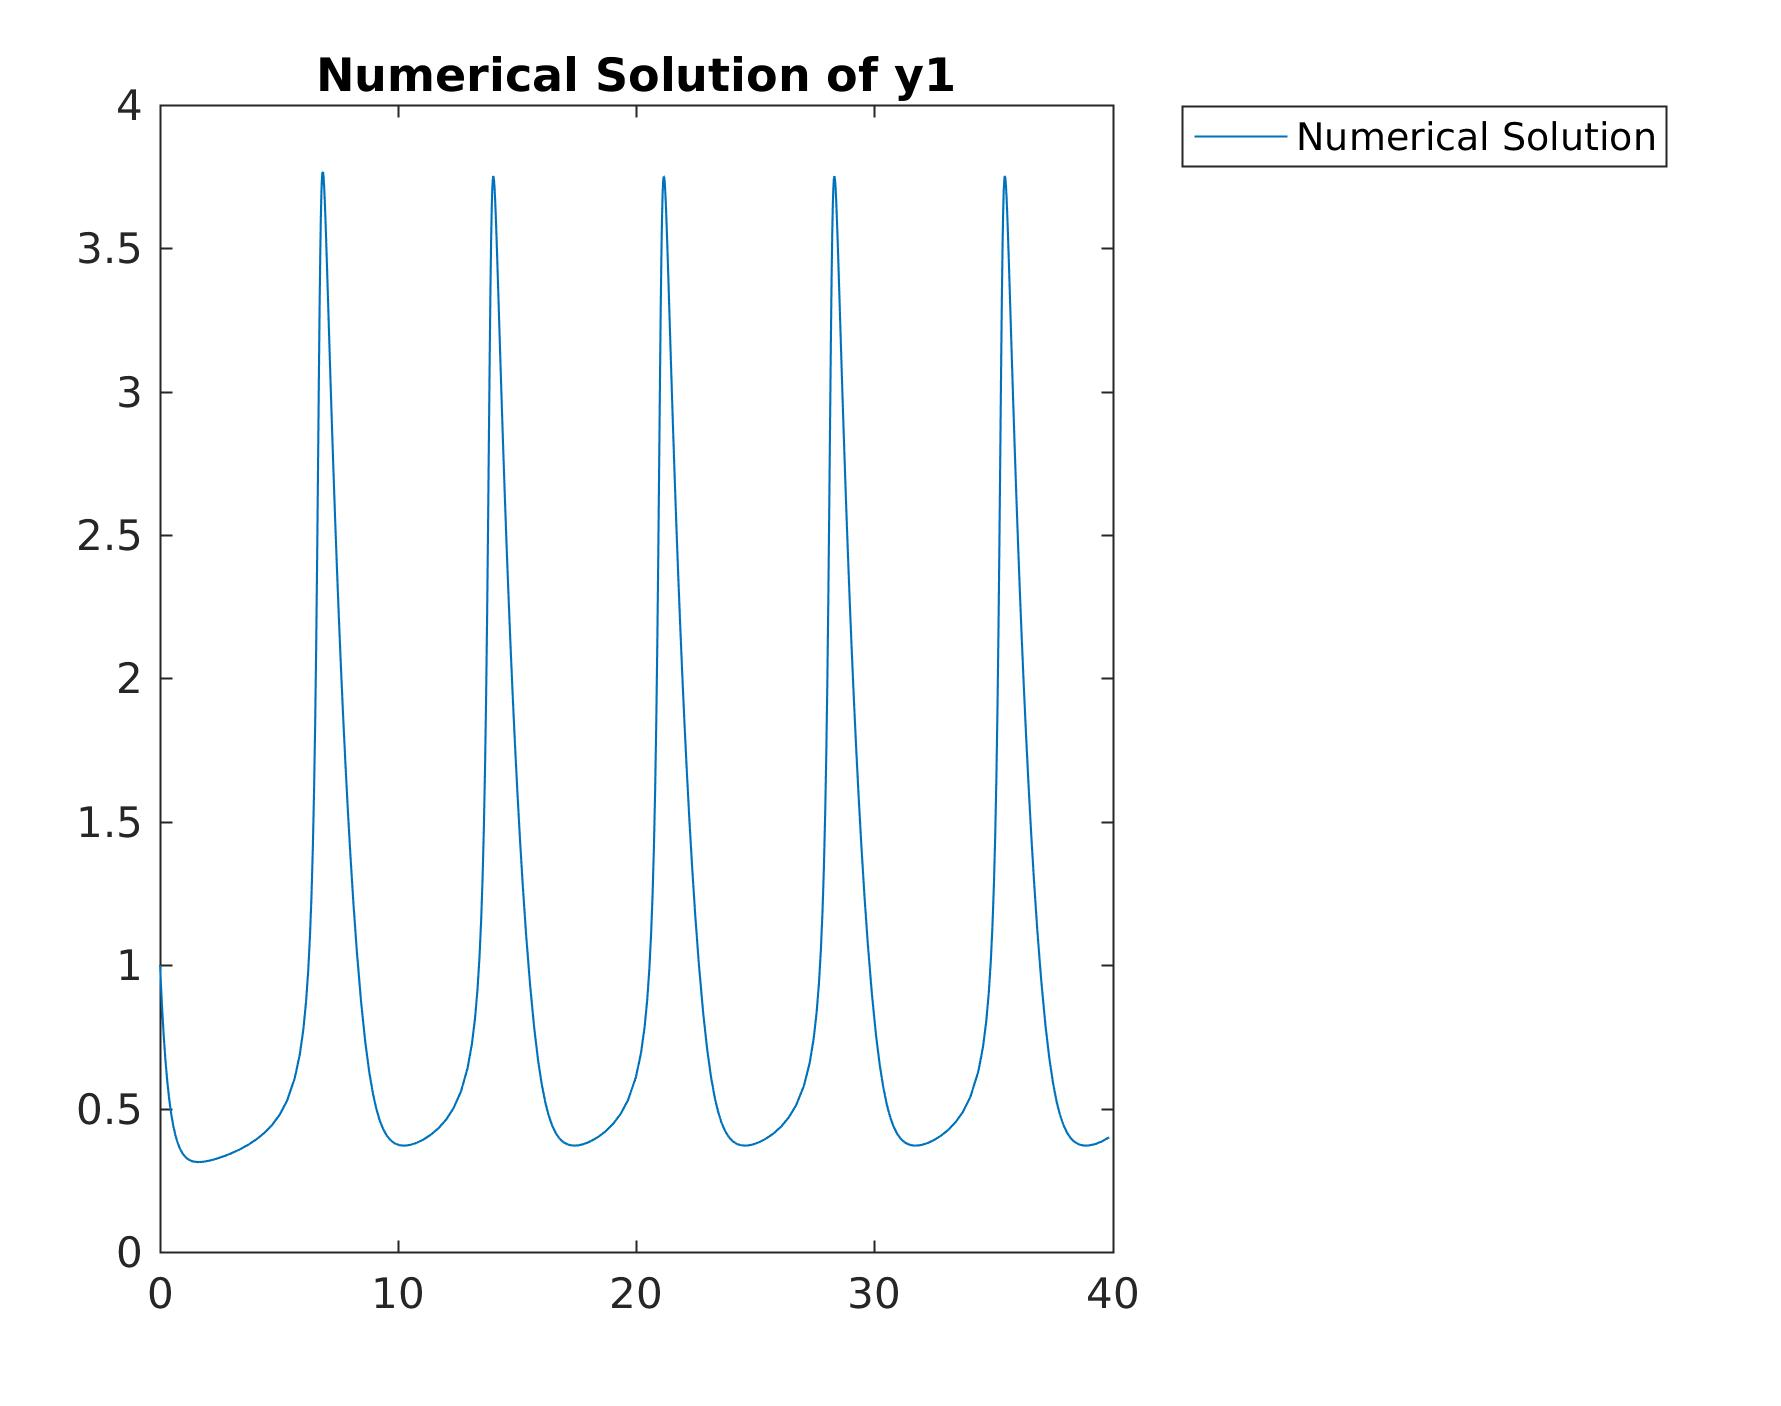
\includegraphics[scale=0.15]{ats_b_y1}
\caption{Using Adaptive Time Steps for Curtiss-Hirschfelder equation.}
\end{figure}
\end{frame}

\begin{frame}
\begin{figure}
\centering
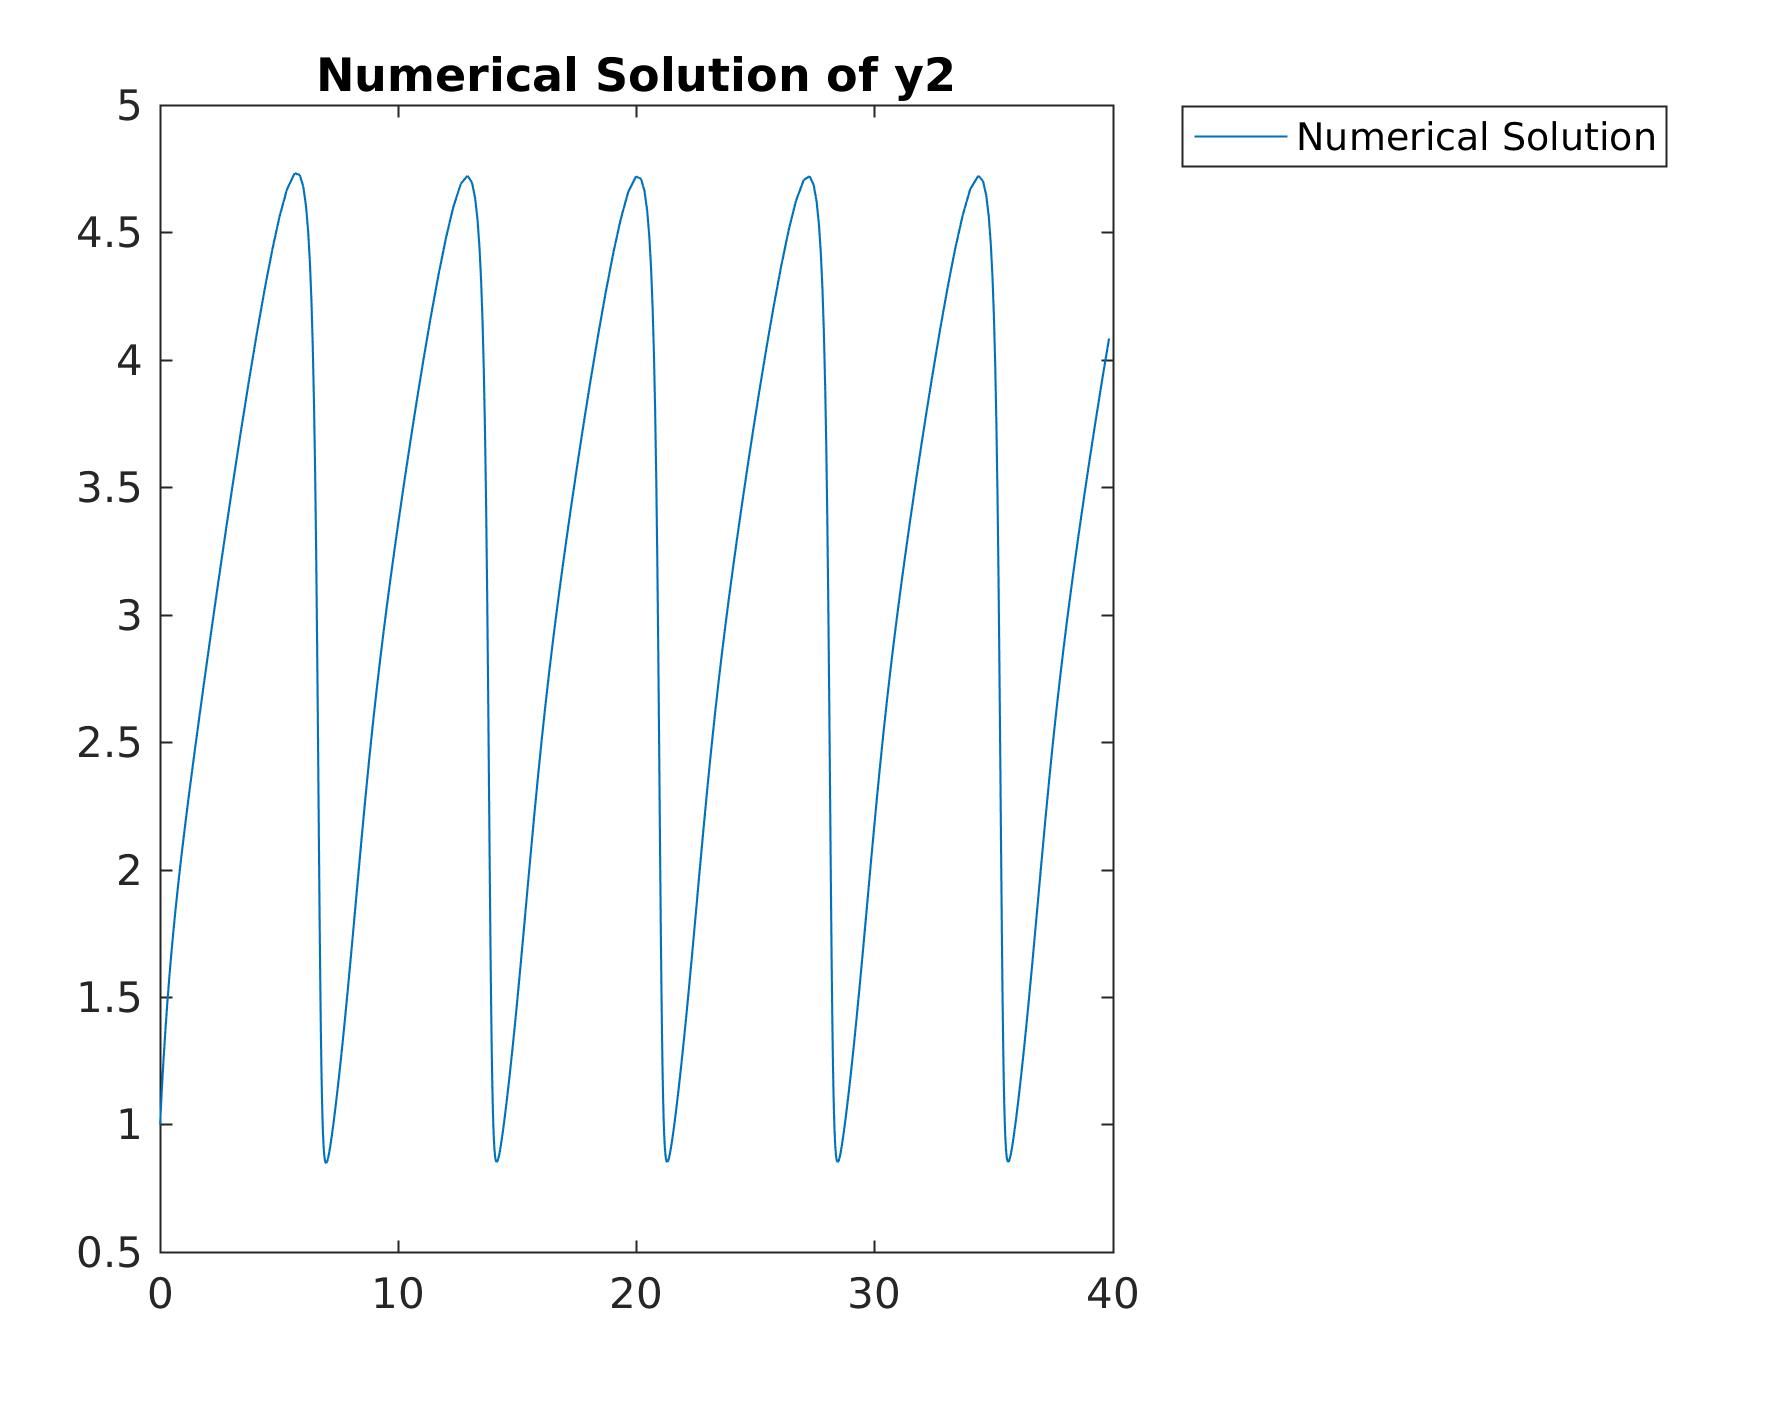
\includegraphics[scale=0.15]{ats_b_y2}
\caption{Using Adaptive Time Steps for Curtiss-Hirschfelder equation.}
\end{figure}
\end{frame}


\begin{frame}{Belousov-Zhabotinsky Reaction (BZ) 2 ODEs}
\textbf{\textsf{Applications.}}
\begin{itemize}
\item A classical example of \textbf{non-equilibrium thermodynamics}, resulting in the establishment of a \textbf{nonlinear chemical oscillator}.
\item An interesting chemical model of \textbf{nonequilibrium biological phenomena}.
\item \textbf{Mathematical models of the BZ reactions} are of theoretical interest and simulations.
\end{itemize}
\begin{block}{Belousov-Zhabotinsky reaction (BZ) 2 ODEs}
\begin{subequations}
\begin{align}
    \frac{dy_1}{dt}  &=  \frac{1}{\epsilon} \left( y_1(1-y_1) + fy_2\frac{q-y_1}{q+y_1} \right)
    \\
    \frac{dy_2}{dt}  &=  y_1-y_2
\end{align}
\end{subequations}
%where $y_1(0) = 0.04$, $y_2(0) = 0.1$,
where the coefficients are given by $f = 2/3$, $q = 8*10^{-4}$ and $\epsilon = 4*10^{-2}$.
%\includepdf[scale=1, pages=-]{bz.pdf}
\end{block}
\end{frame}

\begin{frame}
\begin{figure}
\centering
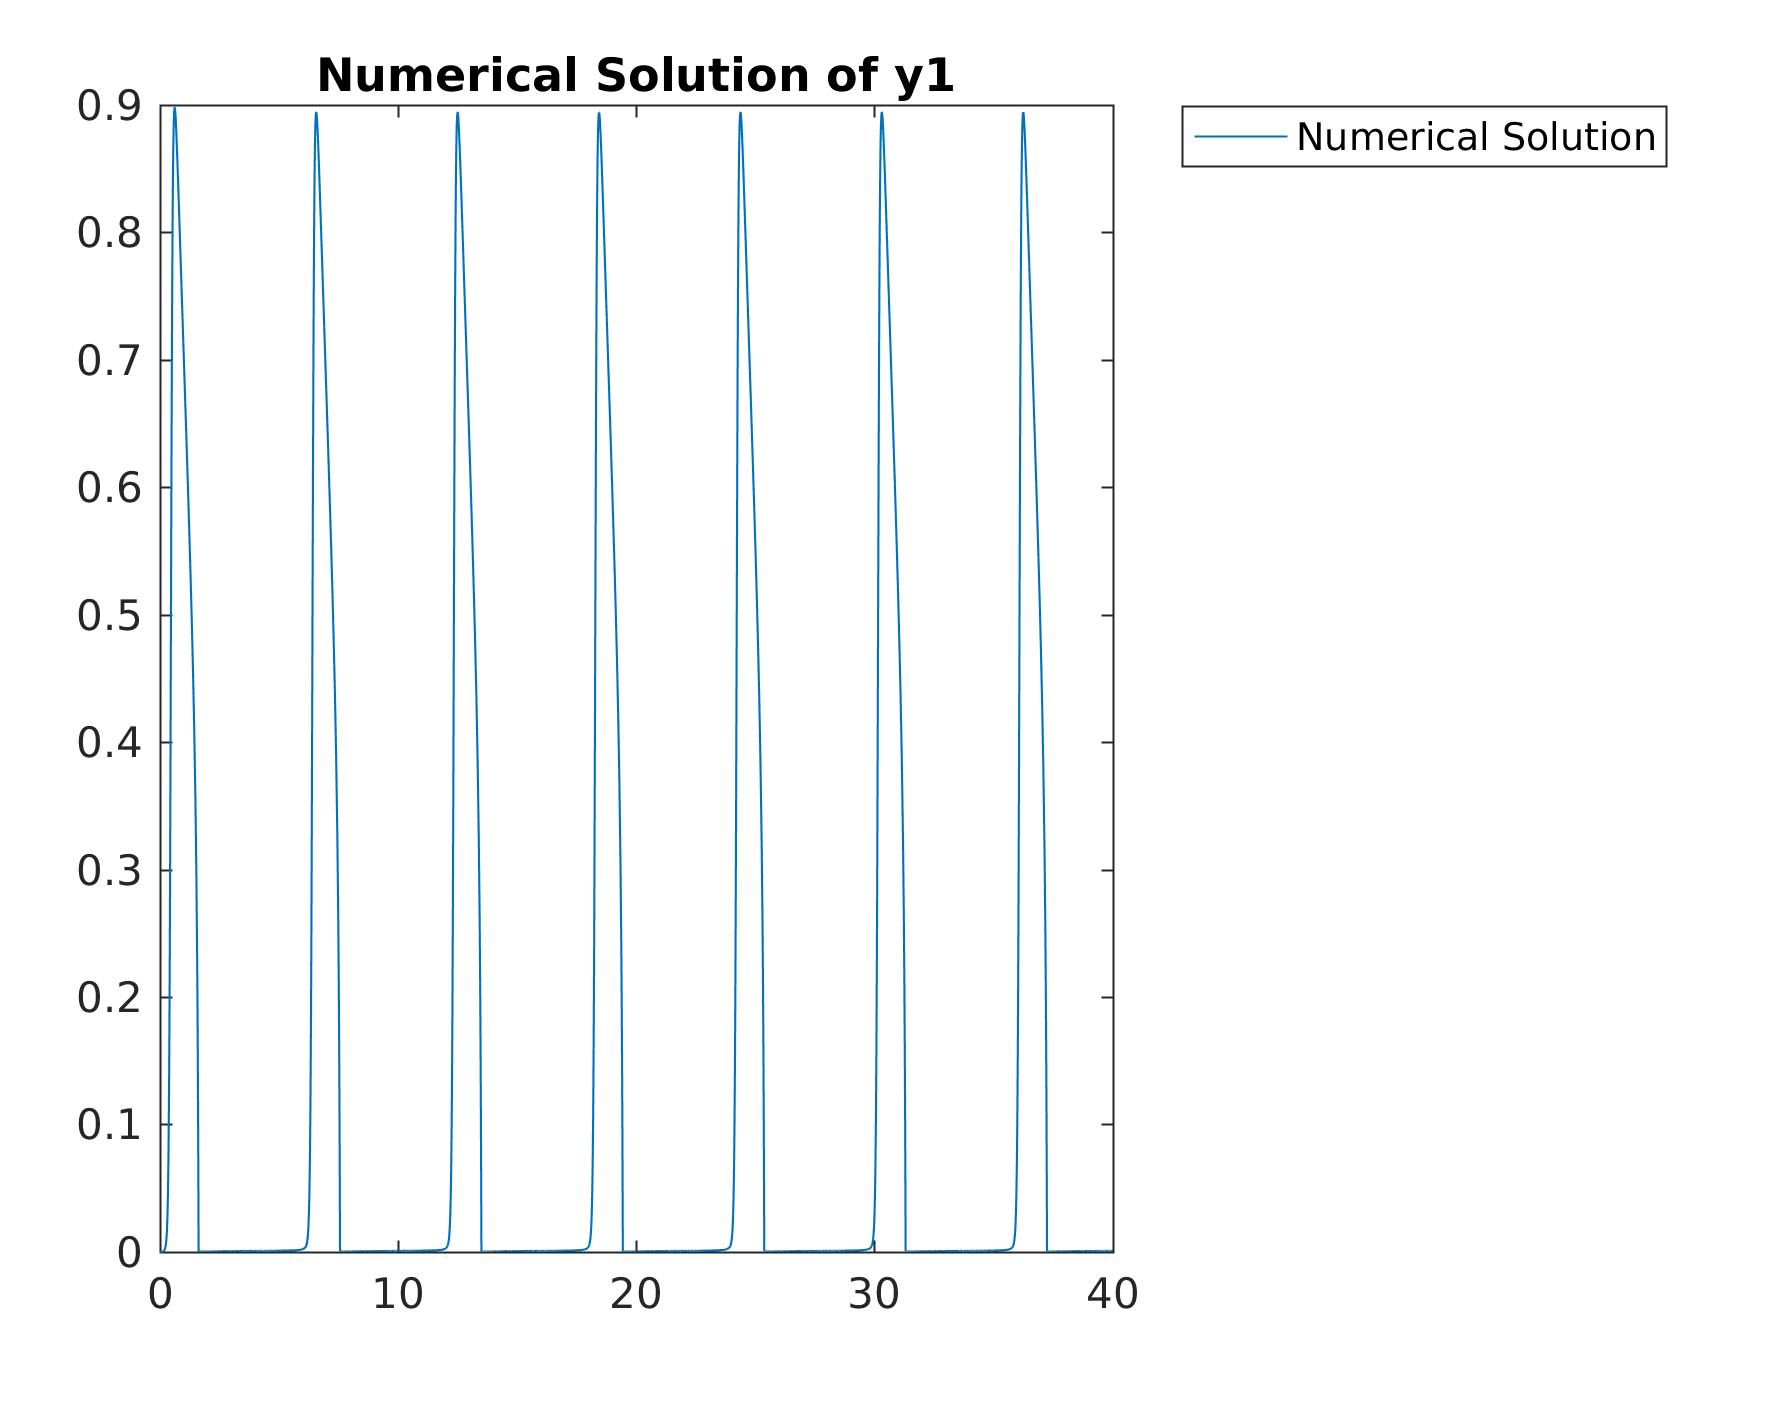
\includegraphics[scale=0.15]{ats_o2_y1}
\caption{Using Adaptive Time Steps for Curtiss-Hirschfelder equation.}
\end{figure}
\end{frame}

\begin{frame}
\begin{figure}
\centering
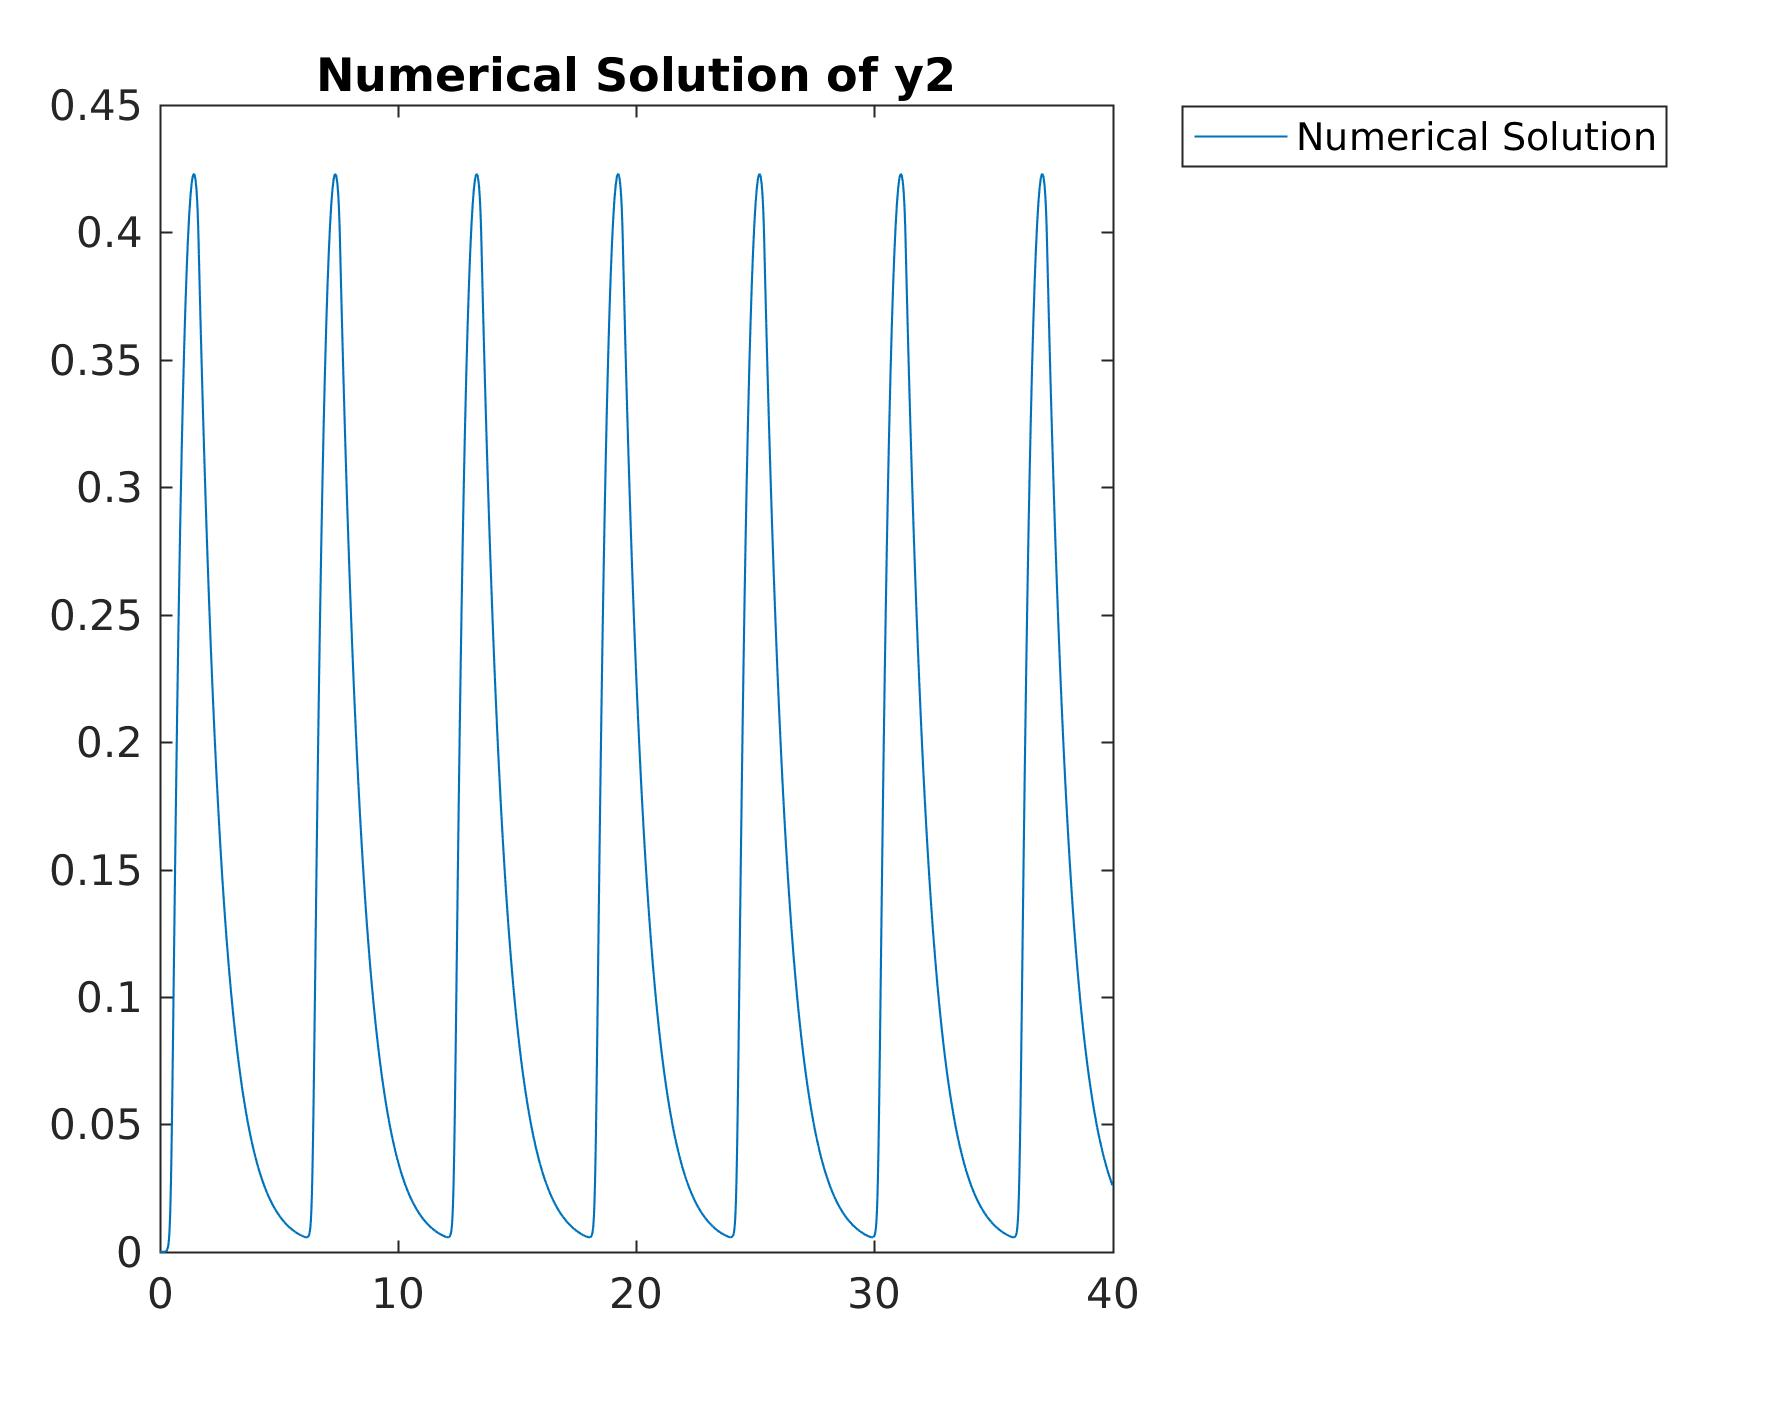
\includegraphics[scale=0.15]{ats_o2_y2}
\caption{Using Adaptive Time Steps for Curtiss-Hirschfelder equation.}
\end{figure}
\end{frame}

\begin{frame}{Oregonator.}
\textbf{\textsf{Applications.}}
\begin{itemize}
\item A theoretical model for a type of \textbf{autocatalytic reaction.}
\item The simplest realistic model of the \textbf{chemical dynamics} of the \textbf{oscillatory Belousov-Zhabotinsky reaction.}
\item A \textbf{reduced model of the FKN mechanism} (developed by Richard Field, Endre K\"{o}r\"{o}s, and Richard M. Noyes).
\end{itemize}
\begin{block}{Oregonator.}
\begin{subequations}
\begin{align}
    \frac{dy_1}{dt}  &=  77.27 \big[y_2  +  y_1 (1 - 8.375*10^{-6} y_1 - y_2) \big]
    \\
    \frac{dy_2}{dt}  &=  \frac{y_3 - (1+y_1)y_2}{77.27}
    , \hspace{0.5cm}
    \frac{dy_3}{dt}  =  0.161(y_1-y_3)
\end{align}
\end{subequations}
where $y_1(0) = 1$, $y_2(0) = 2$ and $y_3(0) = 3$.
%\includepdf[scale=1, pages=-]{ore.pdf}
\end{block}
\end{frame}



\begin{frame}{Belousov-Zhabotinsky reaction (BZ) 3 ODEs}
\begin{block}{Belousov-Zhabotinsky reaction (BZ) 3 ODEs}
\begin{subequations}
\begin{align}
    \frac{dy_1}{dt}  &=  \frac{1}{\mu} (-qy_1 -y_1y_2 + fy_3)
    \\
    \frac{dy_2}{dt}  &=  \frac{1}{\epsilon} (qy_1 -y_1y_2 + y_2 - y_2^2)
    \\
    \frac{dy_3}{dt}  &=  y_2-y_3
\end{align}
\end{subequations}
where $y_1(0) = 10$, $y_2(0) = 0.04$, $y_3(0) = 0.1$,
where the coefficients are given by $f = 2/3$, $q = 8*10^{-4}$, $\mu=10^{-6}$ and $\epsilon = 4*10^{-2}$.
%\includepdf[scale=1, pages=-]{bz3.pdf}
\end{block}
\end{frame}

\begin{frame}
\begin{figure}
\centering
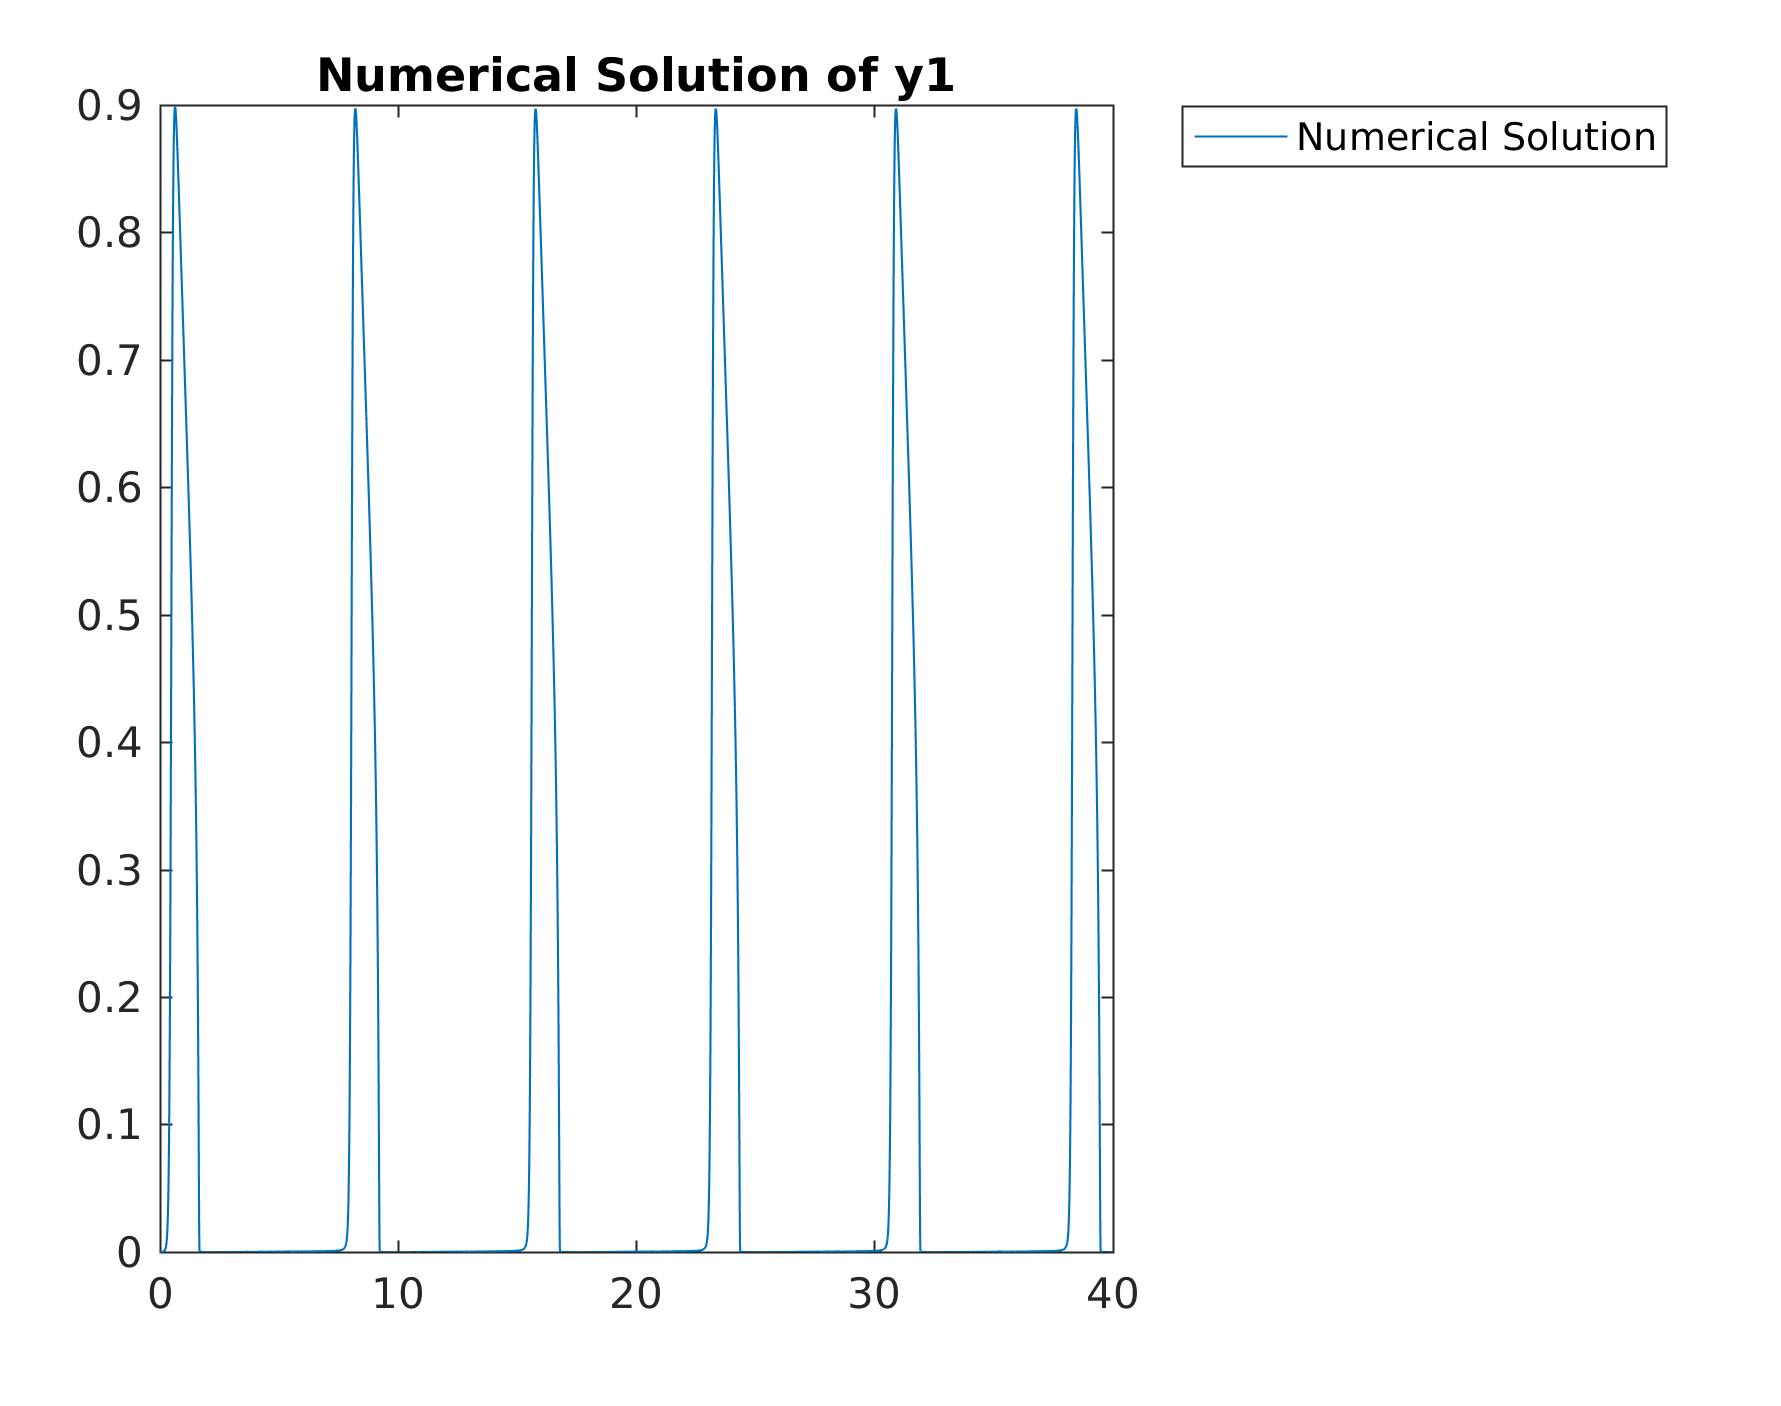
\includegraphics[scale=0.15]{ats_o3_y1}
\caption{Using Adaptive Time Steps for Curtiss-Hirschfelder equation.}
\end{figure}
\end{frame}

\begin{frame}
\begin{figure}
\centering
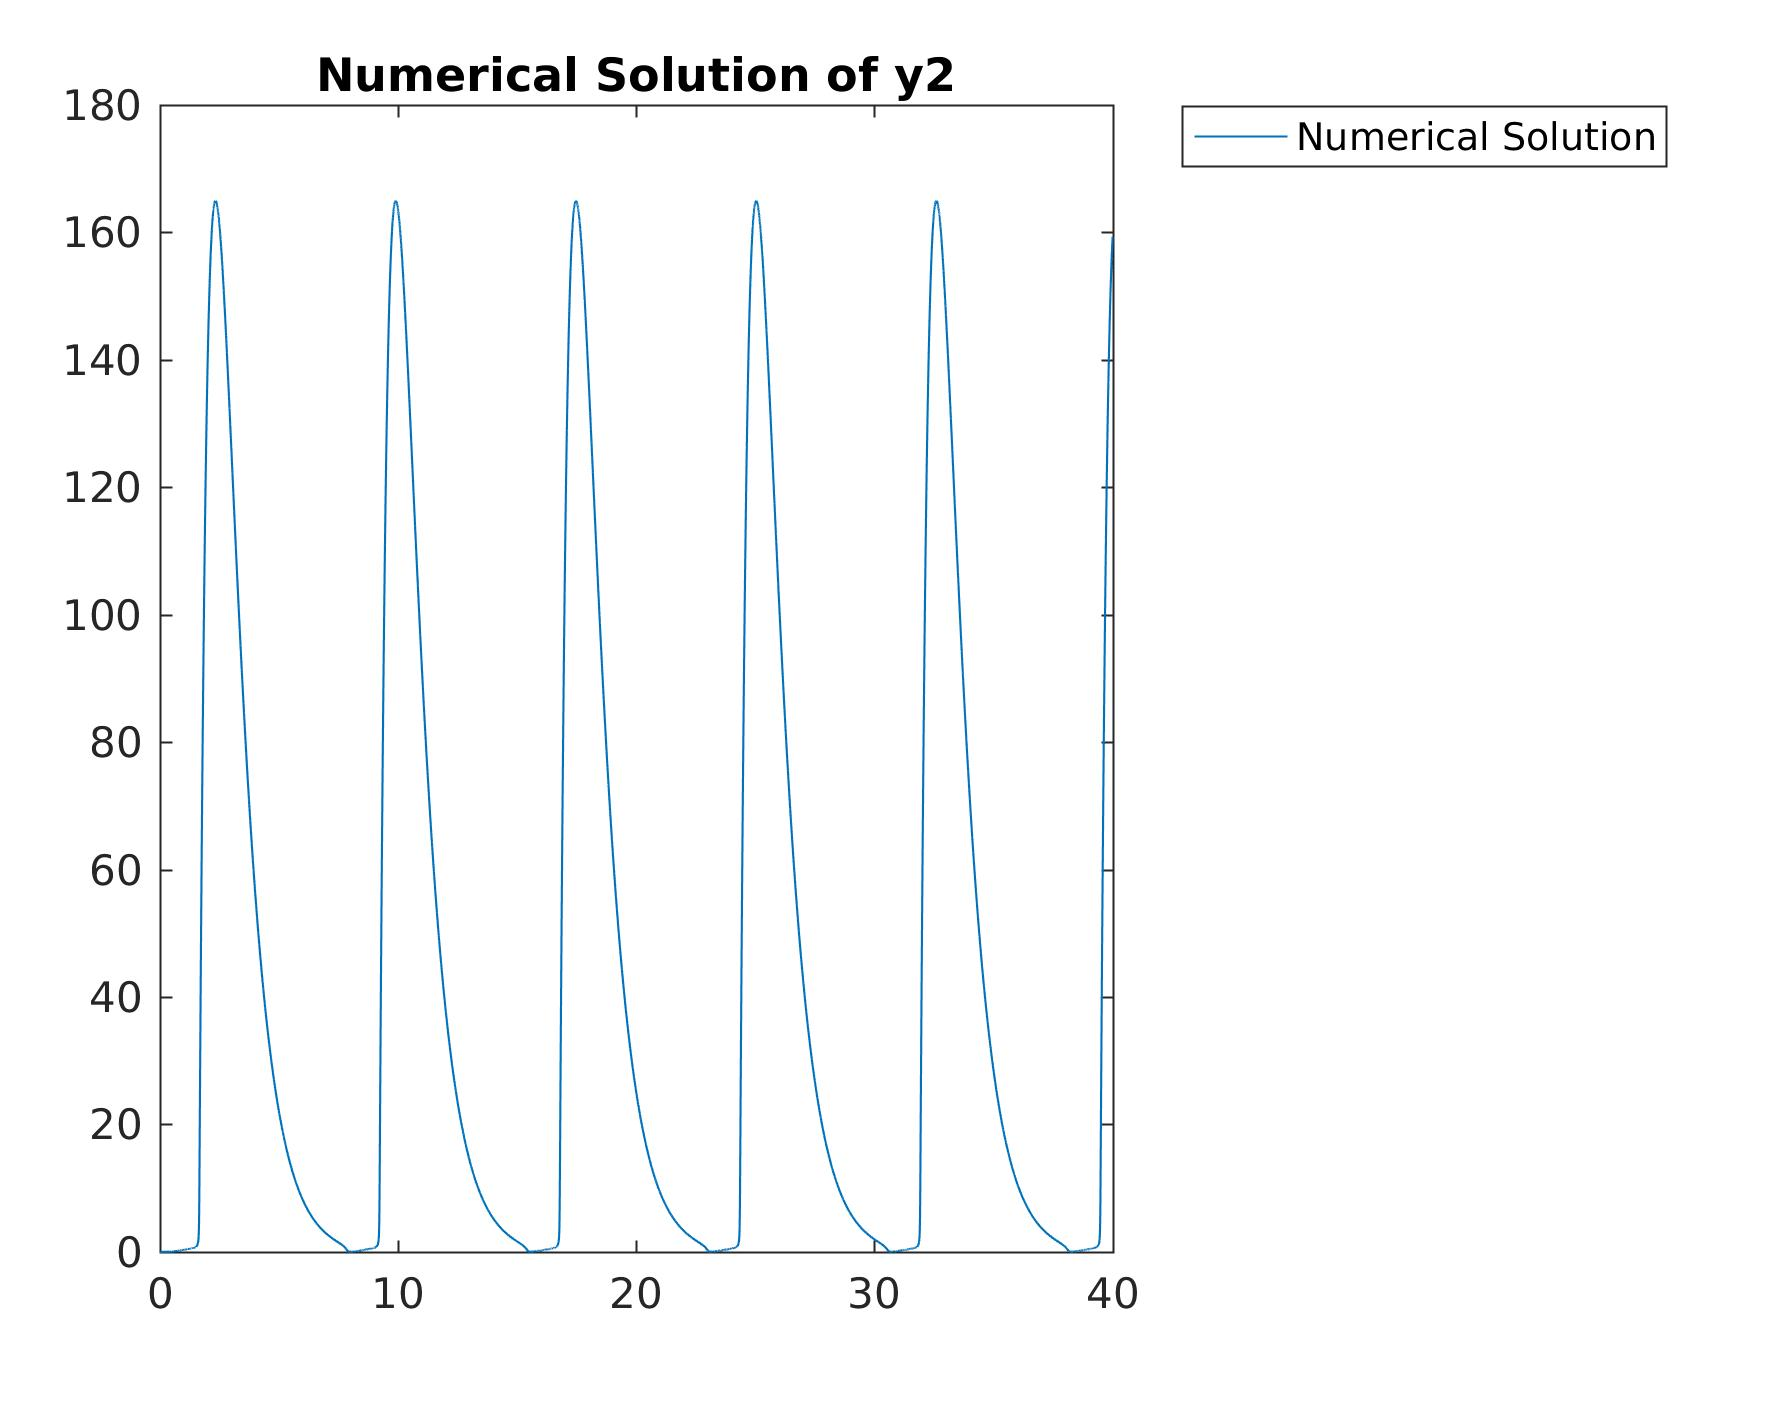
\includegraphics[scale=0.15]{ats_o3_y2}
\caption{Using Adaptive Time Steps for Curtiss-Hirschfelder equation.}
\end{figure}
\end{frame}

\begin{frame}{van der Pol Equations.}
\textbf{\textsf{Applications.}} A basic model for \textbf{oscillatory processes} in physics, electronics, biology, neurology, sociology and economics
\begin{itemize}
\item {\color{blue} \textbf{Physics.}} Models \textbf{electrical circuits connected with triod oscillators}. A prototype for systems with \textbf{self-excited limit cycle oscillations.}
\item {\color{blue} \textbf{Medicine.}} Study the range of \textbf{stability of heart dynamics.} Situation in which a real heart is driven by a pacemaker. Stabilize a \textbf{heart's irregular beating.}
\item {\color{blue} \textbf{Biology.}} The basis of a model of \textbf{coupled neurons in the gastric mill circuit} of the \textbf{stomatogastric ganglion}
\item {\color{blue} \textbf{Seismology.}} Used in the development a model of the \textbf{interaction of two plates} in a \textbf{geological fault.}
\end{itemize}
\begin{block}{van der Pol equations}
\begin{subequations}
\begin{align}
    \frac{dy_1}{dt}  &=  y_2
    \\
    \frac{dy_2}{dt}  &=  [ (1-y_1^2)y_2 - y_1 ] / \epsilon
\end{align}
\end{subequations}
where $\epsilon = 10^{-6}$.
\end{block}
\end{frame}

\begin{frame}
\begin{figure}
\centering
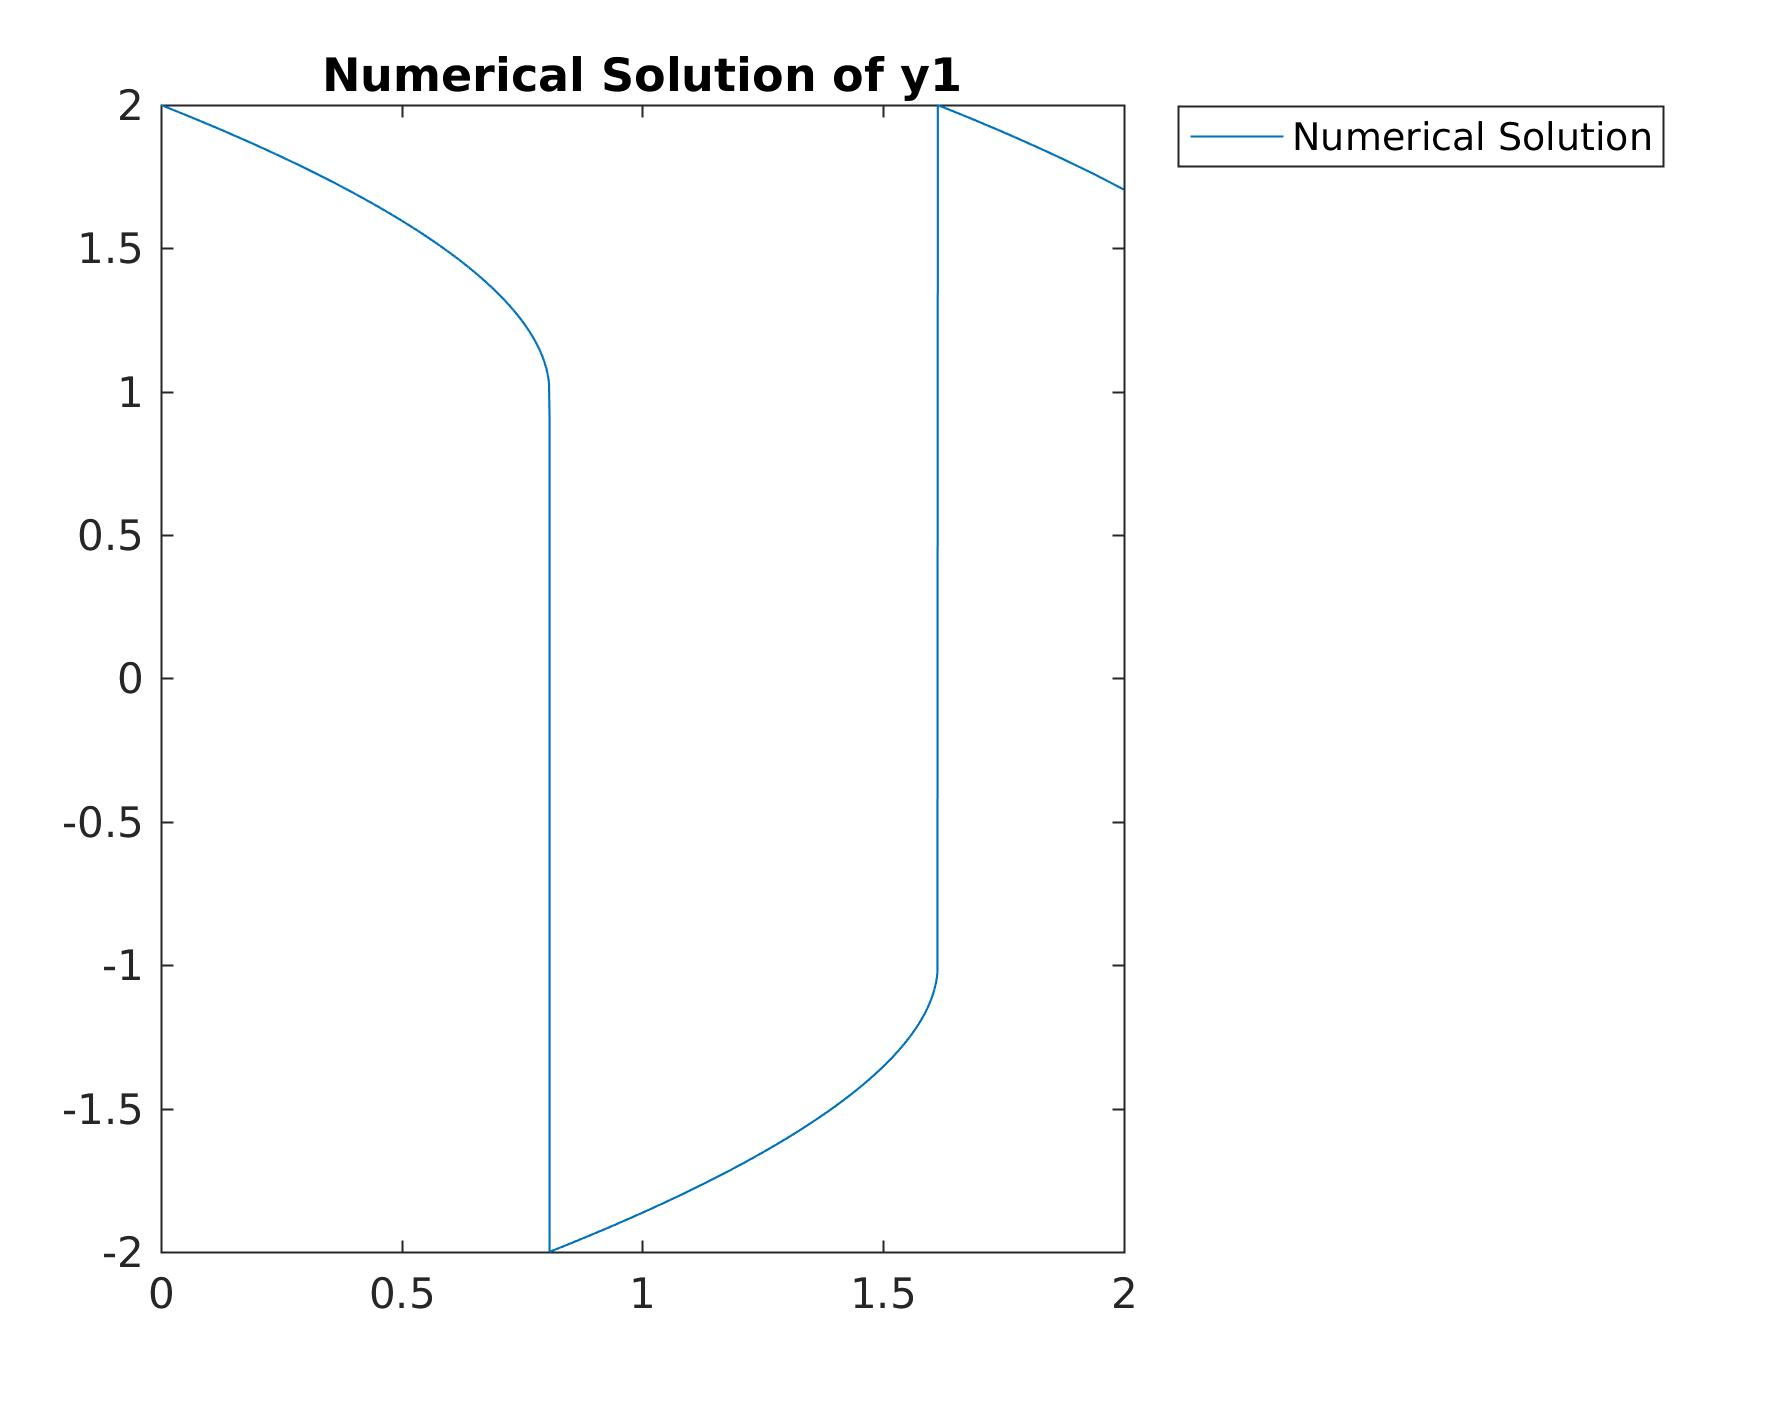
\includegraphics[scale=0.15]{ats_vdp_y1}
\caption{Using Adaptive Time Steps for Curtiss-Hirschfelder equation.}
\end{figure}
\end{frame}
\begin{frame}
\begin{figure}
\centering
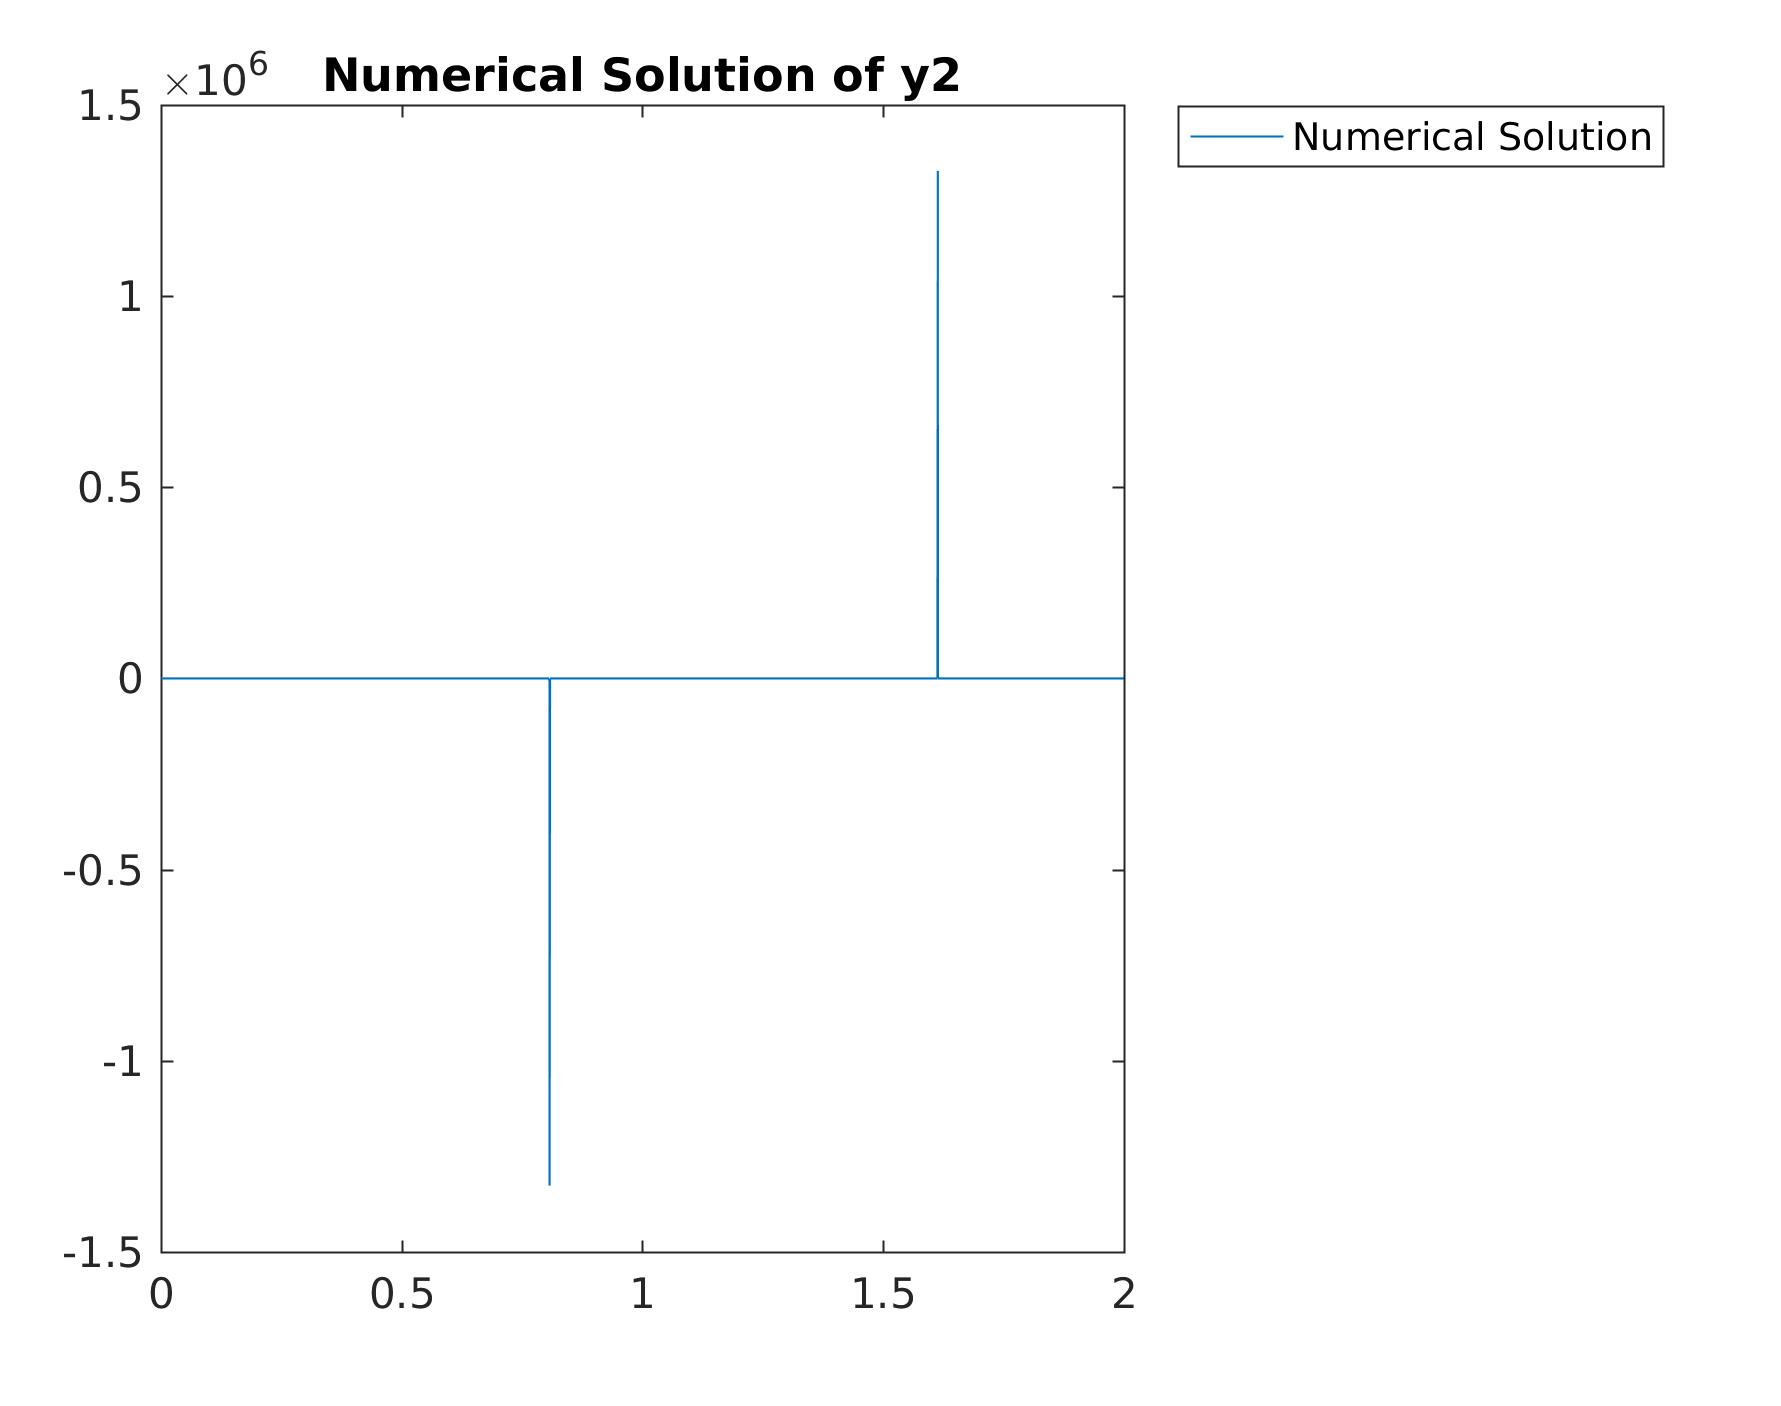
\includegraphics[scale=0.15]{ats_vdp_y2}
\caption{Using Adaptive Time Steps for Curtiss-Hirschfelder equation.}
\end{figure}
\end{frame}



\begin{frame}{References}
\textbf{References}
\begin{thebibliography}{999}
\bibitem {1} Tan Trung Nguyen, Frédérique Laurent, Rodney Fox, Marc Massot. \textit{Solution of population
balance equations in applications with fine particles: mathematical modeling and numerical
schemes}. 2016. $<$hal-01247390v2$>$
\end{thebibliography}

\end{frame}



\end{document}